\section{Architecture}
\label{sec:architecture}
This section outlines the architecture of the Votes-System.
At first, we elaborate the design of its EJB-Module.
Following that, we briefly discuss the architecture of the War-Module.


\subsection{VotesEJB Architecture}
\label{subsec:votesejb-architector}
In order to maintain scalability, the business and persistence components of a JavaEE Web Application are packaged into an EJB JAR module.
Such modules can easily be cloned to handle more workload properly.
In general an EJB module consists of an domain model, an arbitrary amount of business and persistence classes and a facade, making the relevant components visible to the outside.

\subsubsection{The Votes Domain Model}
\label{subsubsec:the-votes-domain-model}
The Votes Domain Model specifies the structure and relations of its entities.
It is depicted in figure \ref{figure:ejb-model} and mostly matches the requirements defined in section §\ref{sec:requirements}.
However, we made some extensions:

\begin{figure}[h]
\centering
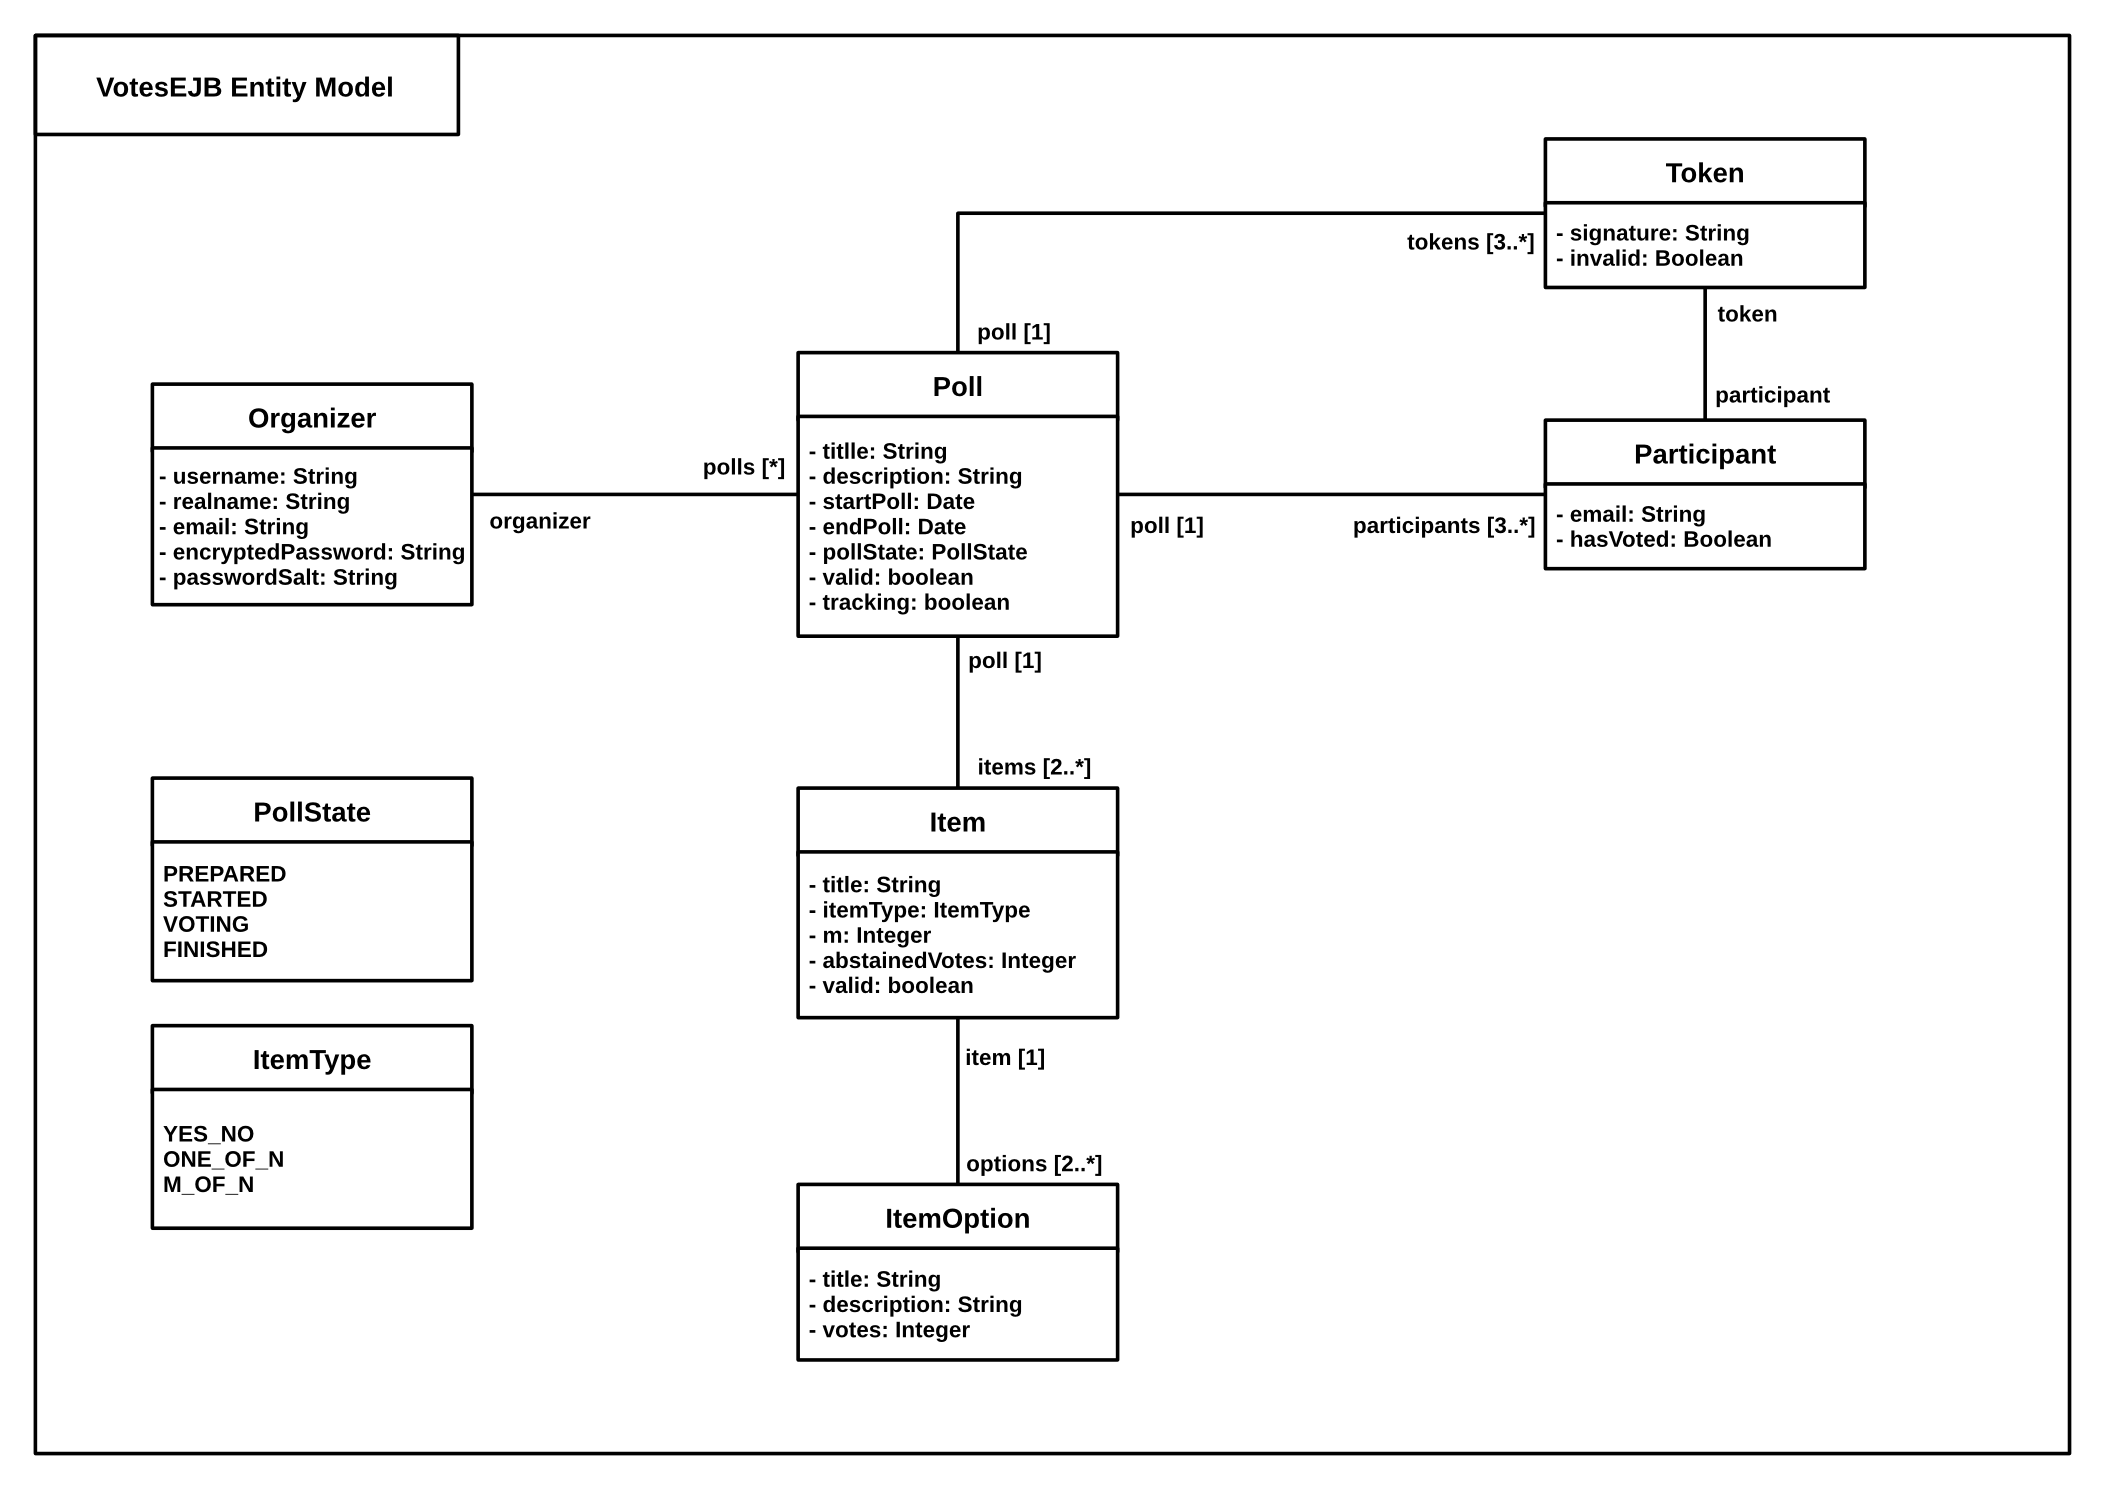
\includegraphics[width=0.7\textwidth]{png/ejb-model.png}
\caption{VotesEJB Entity Model}
\label{figure:ejb-model}
\end{figure}

\begin{itemize}

\item
Polls and Items have flag, which determines if they are valid.

\item
Items have a counter for abstentions.

\item
ItemOptions have a counter that represents the number of participants who have selected the corresponding option.

\item
Tokens can be invalidated.

\item
Organizers also store a salt to strengthen password hashes.

\end{itemize}



\paragraph{Anonymity:}
The criterion of utmost importance for a voting system's quality is the degree of assured anonymity.
That means, at no point it must be possible to link a participant to his or hers voting decision.
Therefore certain restriction have been made:
\begin{itemize}

\item
Polls with less than three participants cannot be asserted anonymous, so poll has to have at least three participants.

\item
Although the voting system records which participant has voted for administrative purposes, his or hers exact vote remains unknown to the data structure.
This is ensured by numeric option counters, which increase if a participant has selected an option.

\item
Token signatures act as ballots, which allow a participant to view polls and submit a vote. 
Such signatures must be hard to forge.
To assure this quality, signatures are type 4 UUIDs generated by \texttt{UUID.randomUUID()}\footnote{\url{http://docs.oracle.com/javase/7/docs/api/java/util/UUID.html}}.

\end{itemize}


\paragraph{Security:}
Another issue of importance is reflected by the domain model is the authentication of organizers.
To ensure that only the creators of polls can access their settings, organizer passwords cannot be stored in clear text.
In order to secure the database against attacks, we facilitate the common technique of salted hashes to store passwords.
A password is stored as SHA-256 hash of its concatenation with a type 4 UUID salt.
The salt is stored alongside.


\subsubsection{Votes Entity Persistence}
\label{subsubsec:votes-entity-persistence}
The Java Persistence API (JPA) used by JavaEE Web Applications follow a persistence strategy, which maps entity classes to database tables.
That means for each entity in the domain model exists a corresponding table.
However, to ensure the uniqueness of row tuples, entities need to have an \texttt{id} property, which is missing in figure \ref{figure:ejb-model}.
Entities of the votes domain model inherit such a property from the class AbstractEntity, depicted in figure \ref{figure:ejb-abstract-entity}.

\begin{figure}[h]
\centering
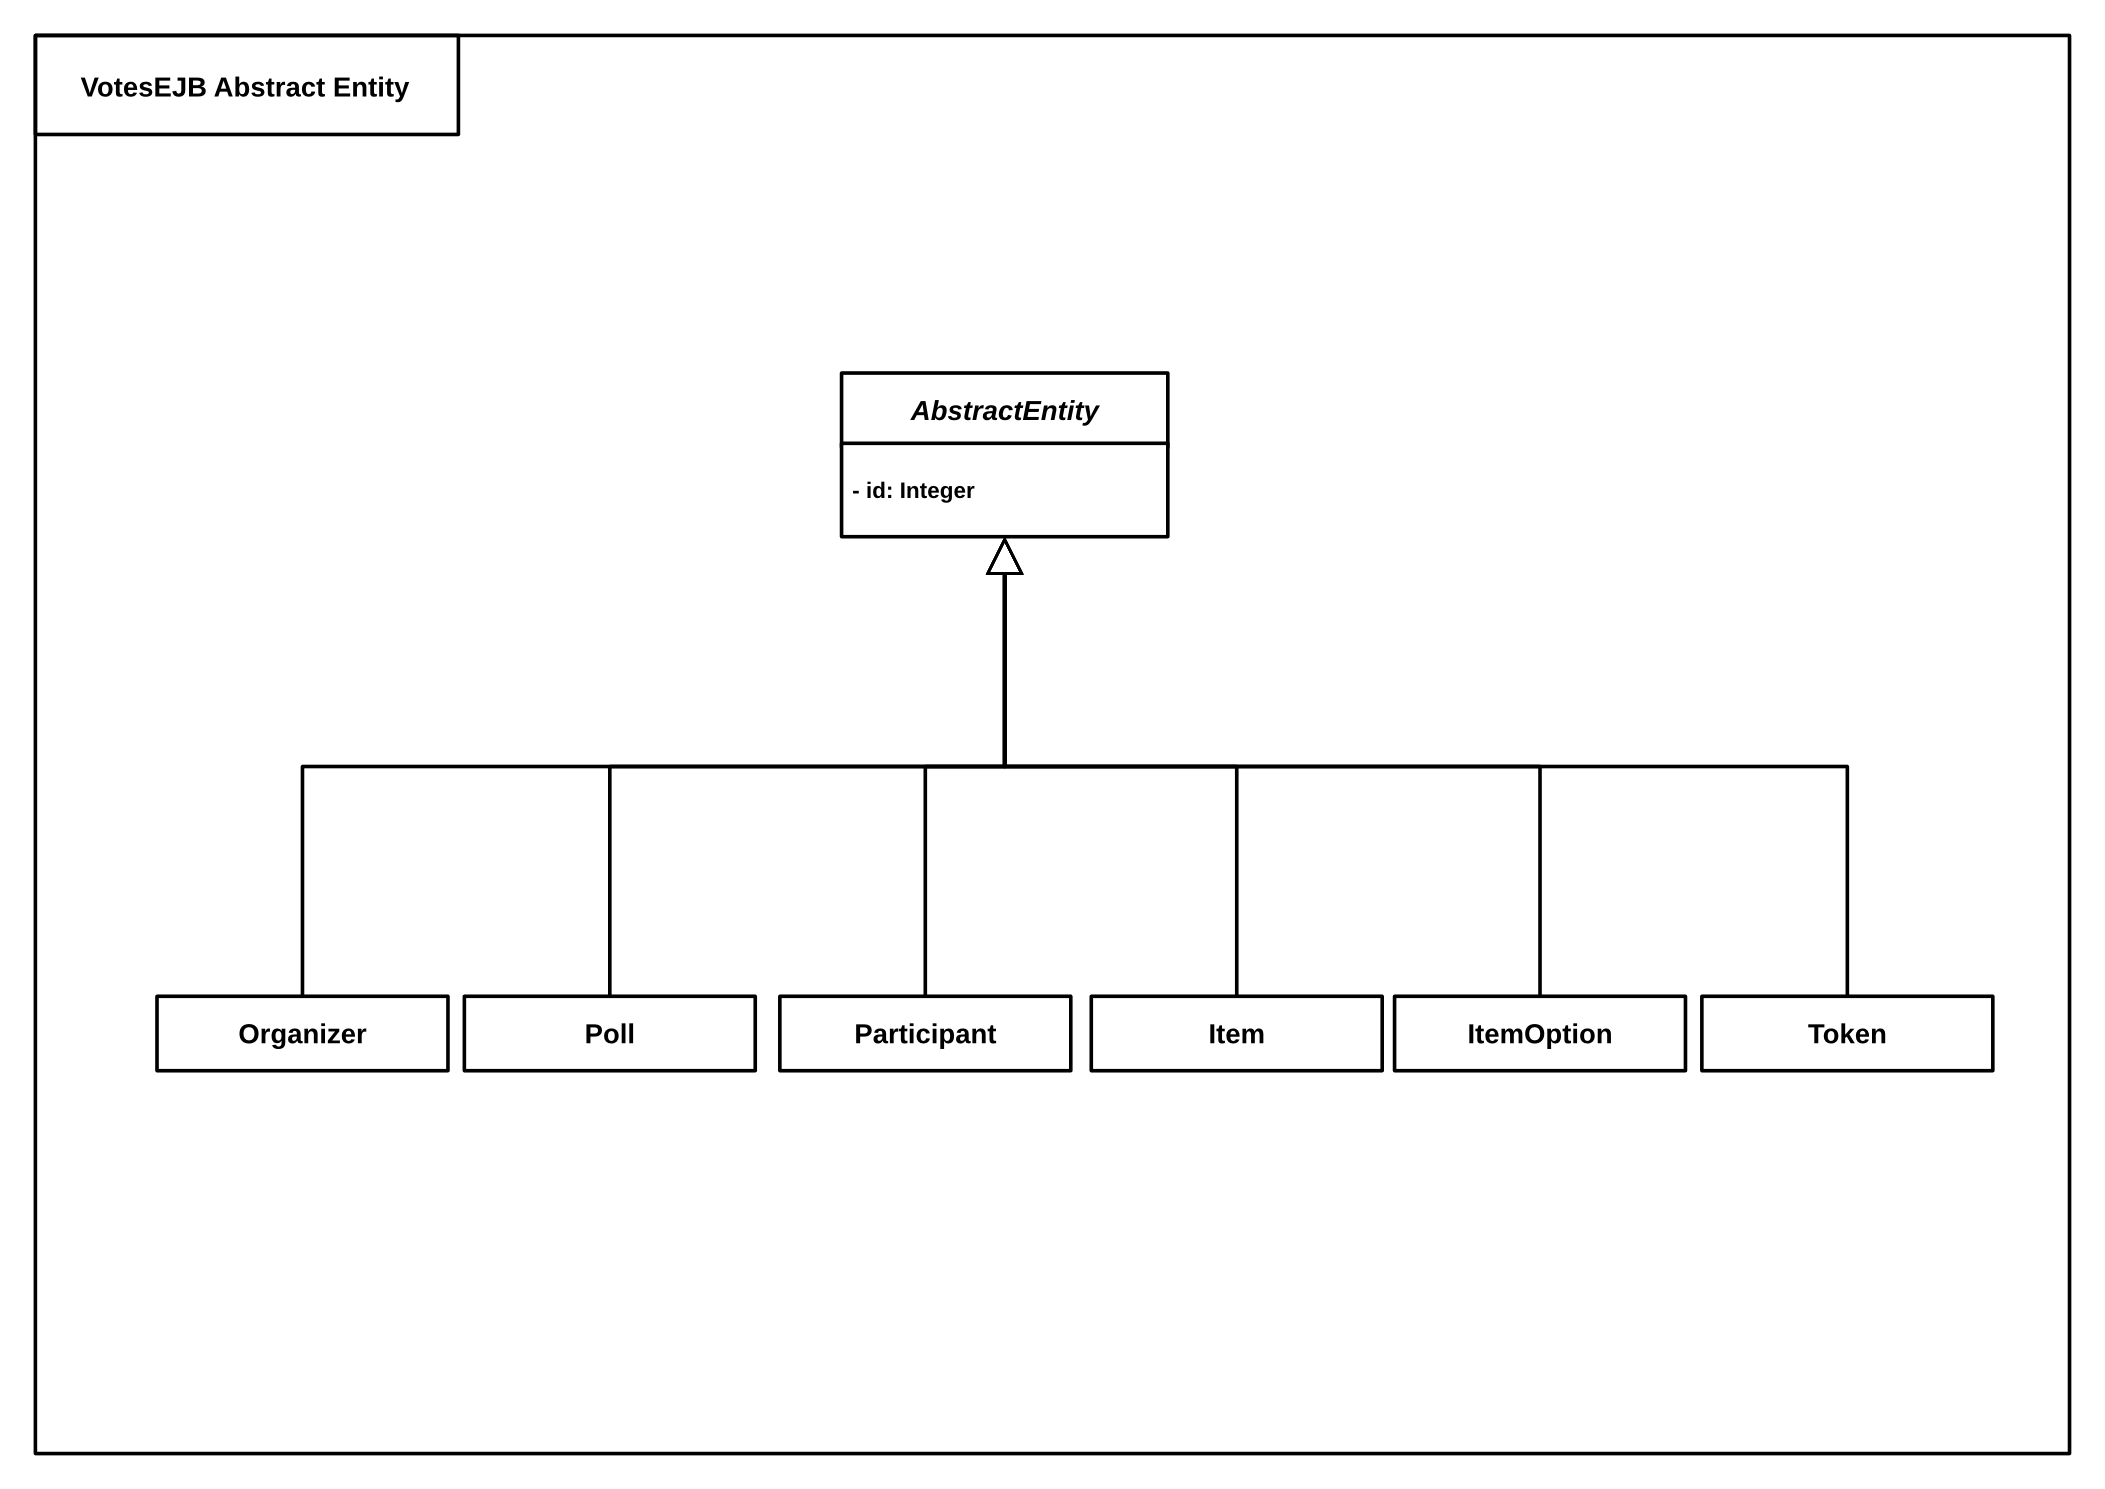
\includegraphics[width=0.7\textwidth]{png/ejb-abstract-entity.png}
\caption{VotesEJB Abstract Entity}
\label{figure:ejb-abstract-entity}
\end{figure}

Moreover, JPA encourages to use the \textit{Data Mapper}\footnote{\url{http://martinfowler.com/eaaCatalog/dataMapper.html}} pattern to handle persistence operations.
This pattern is exemplified in figure \ref{figure:ejb-data-mapper}, which shows the Poll entity class and its corresponding data mapper PollAccess.

\begin{figure}[h]
\centering
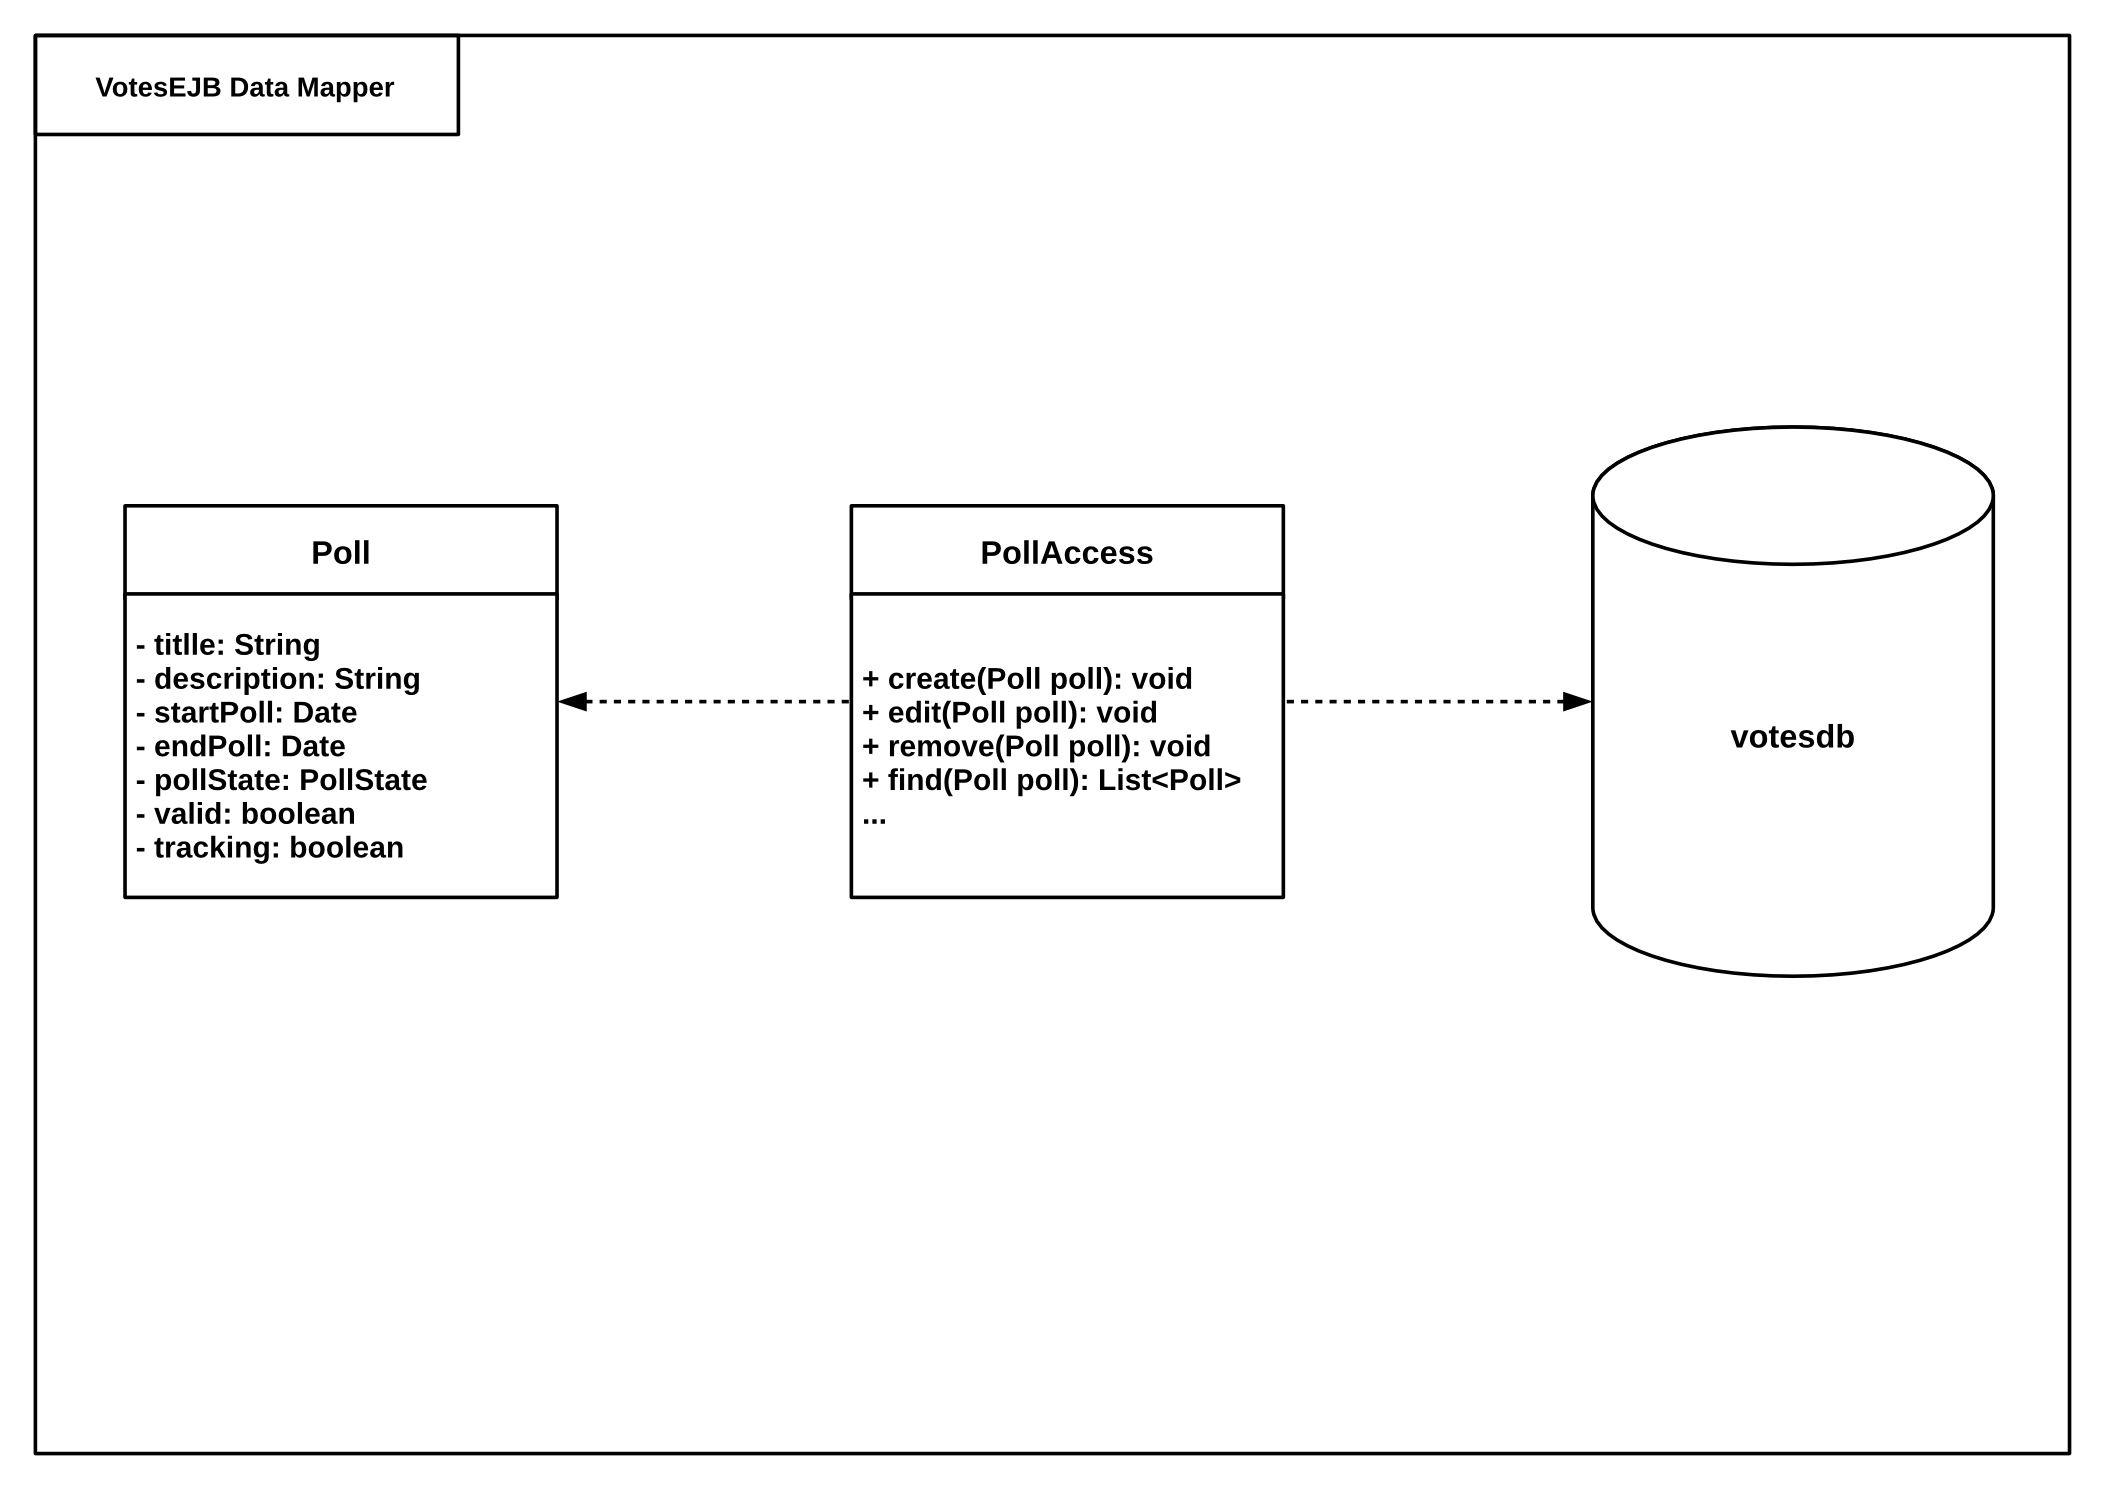
\includegraphics[width=0.7\textwidth]{png/ejb-data-mapper.png}
\caption{VotesEJB Data Mapper}
\label{figure:ejb-data-mapper}
\end{figure}

Each entity of the votes domain model has its own data mapper handling creation, reading, update and deletion of instances in the database.
Thus, this pattern decouples persistence structure from persistence behaviour. 
Mappers or Data Access Objects are also enhanced to do more complex database operations.

\subsubsection{The Votes Business Model}
\label{subsubsec:the-votes-business-model}
Besides the CRUD operations of the persistence layer, the Votes-System has scarcely any business logic.
One notable exception is the transition of poll states depicted in figure \ref{figure:poll-states}.

\begin{figure}[h]
\centering
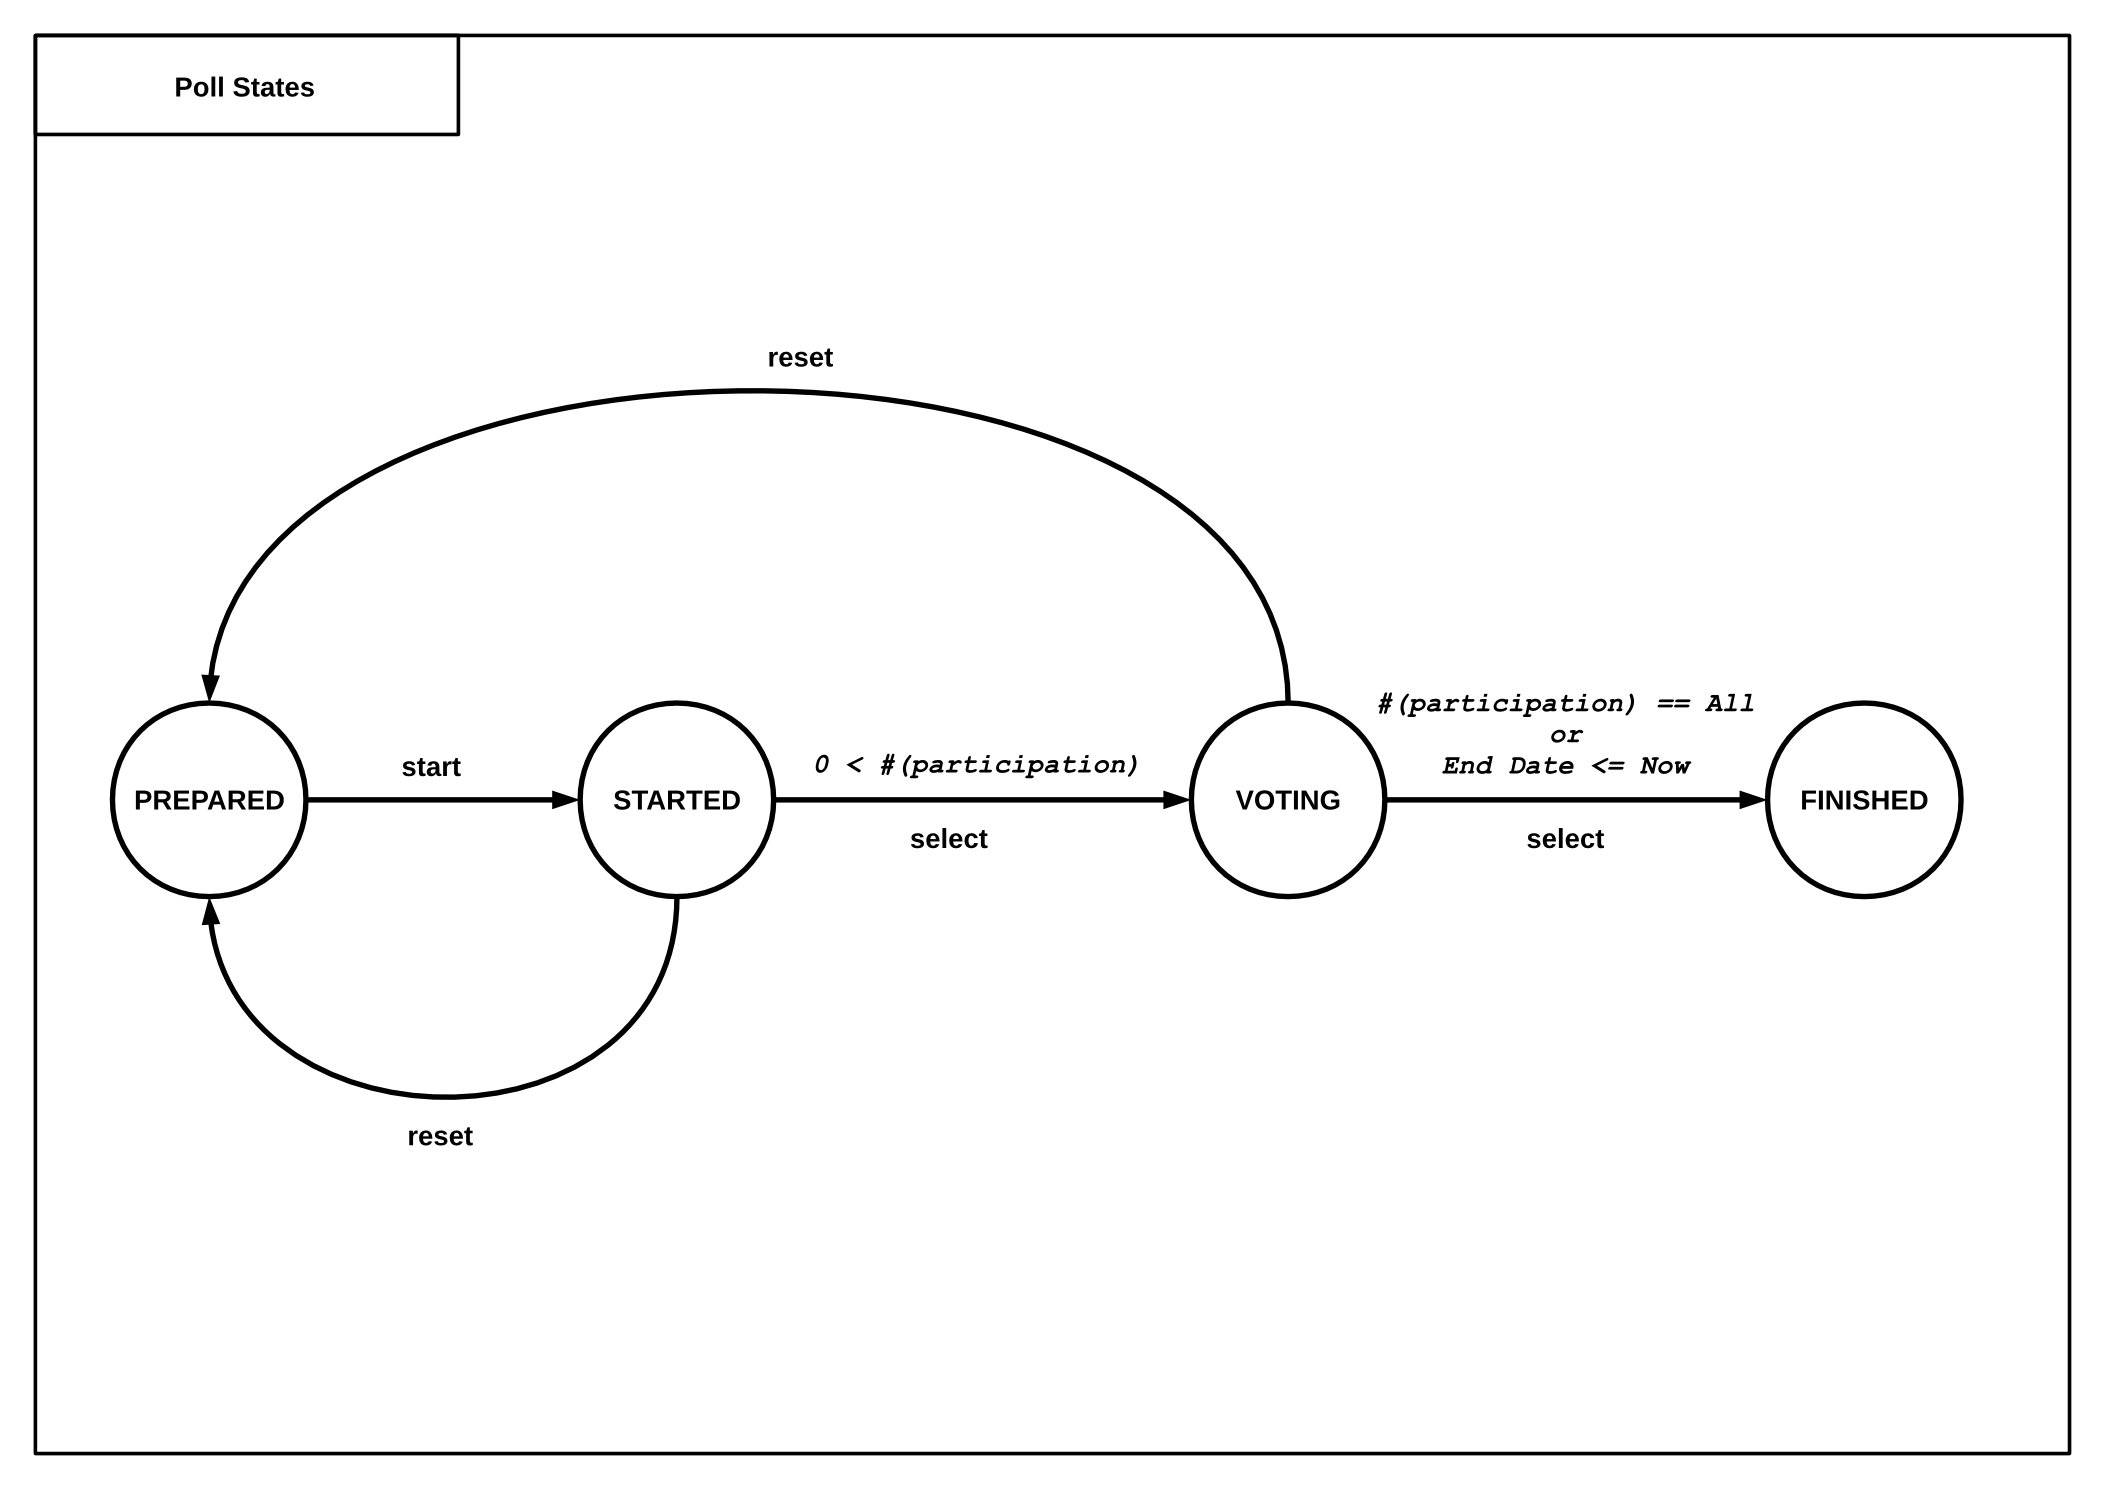
\includegraphics[width=0.7\textwidth]{png/poll-states.png}
\caption{Poll States}
\label{figure:poll-states}
\end{figure}

Poll states are frequently updated when either an organizer or participant access a certain poll.
Per default, a poll is created in state \texttt{PREPARED}.
If its organizer actively starts the poll, the state changes to \texttt{STARTED}.
This will trigger the sending of notification mails to all participants.
As soon as the first participant has submitted his or her vote the poll state changes to \texttt{VOTING}.
In either poll state \texttt{STARTED} or \texttt{VOTING} the organizer can reset the poll.
However, this will result in the deletion of all submitted votes so far.
When all participants have submitted their votes or the poll period is expired, the poll state changes to \texttt{FINISHED}.
This is the final state of poll.
If this state is reached, no further modification is possible.

\begin{figure}[h]
\centering
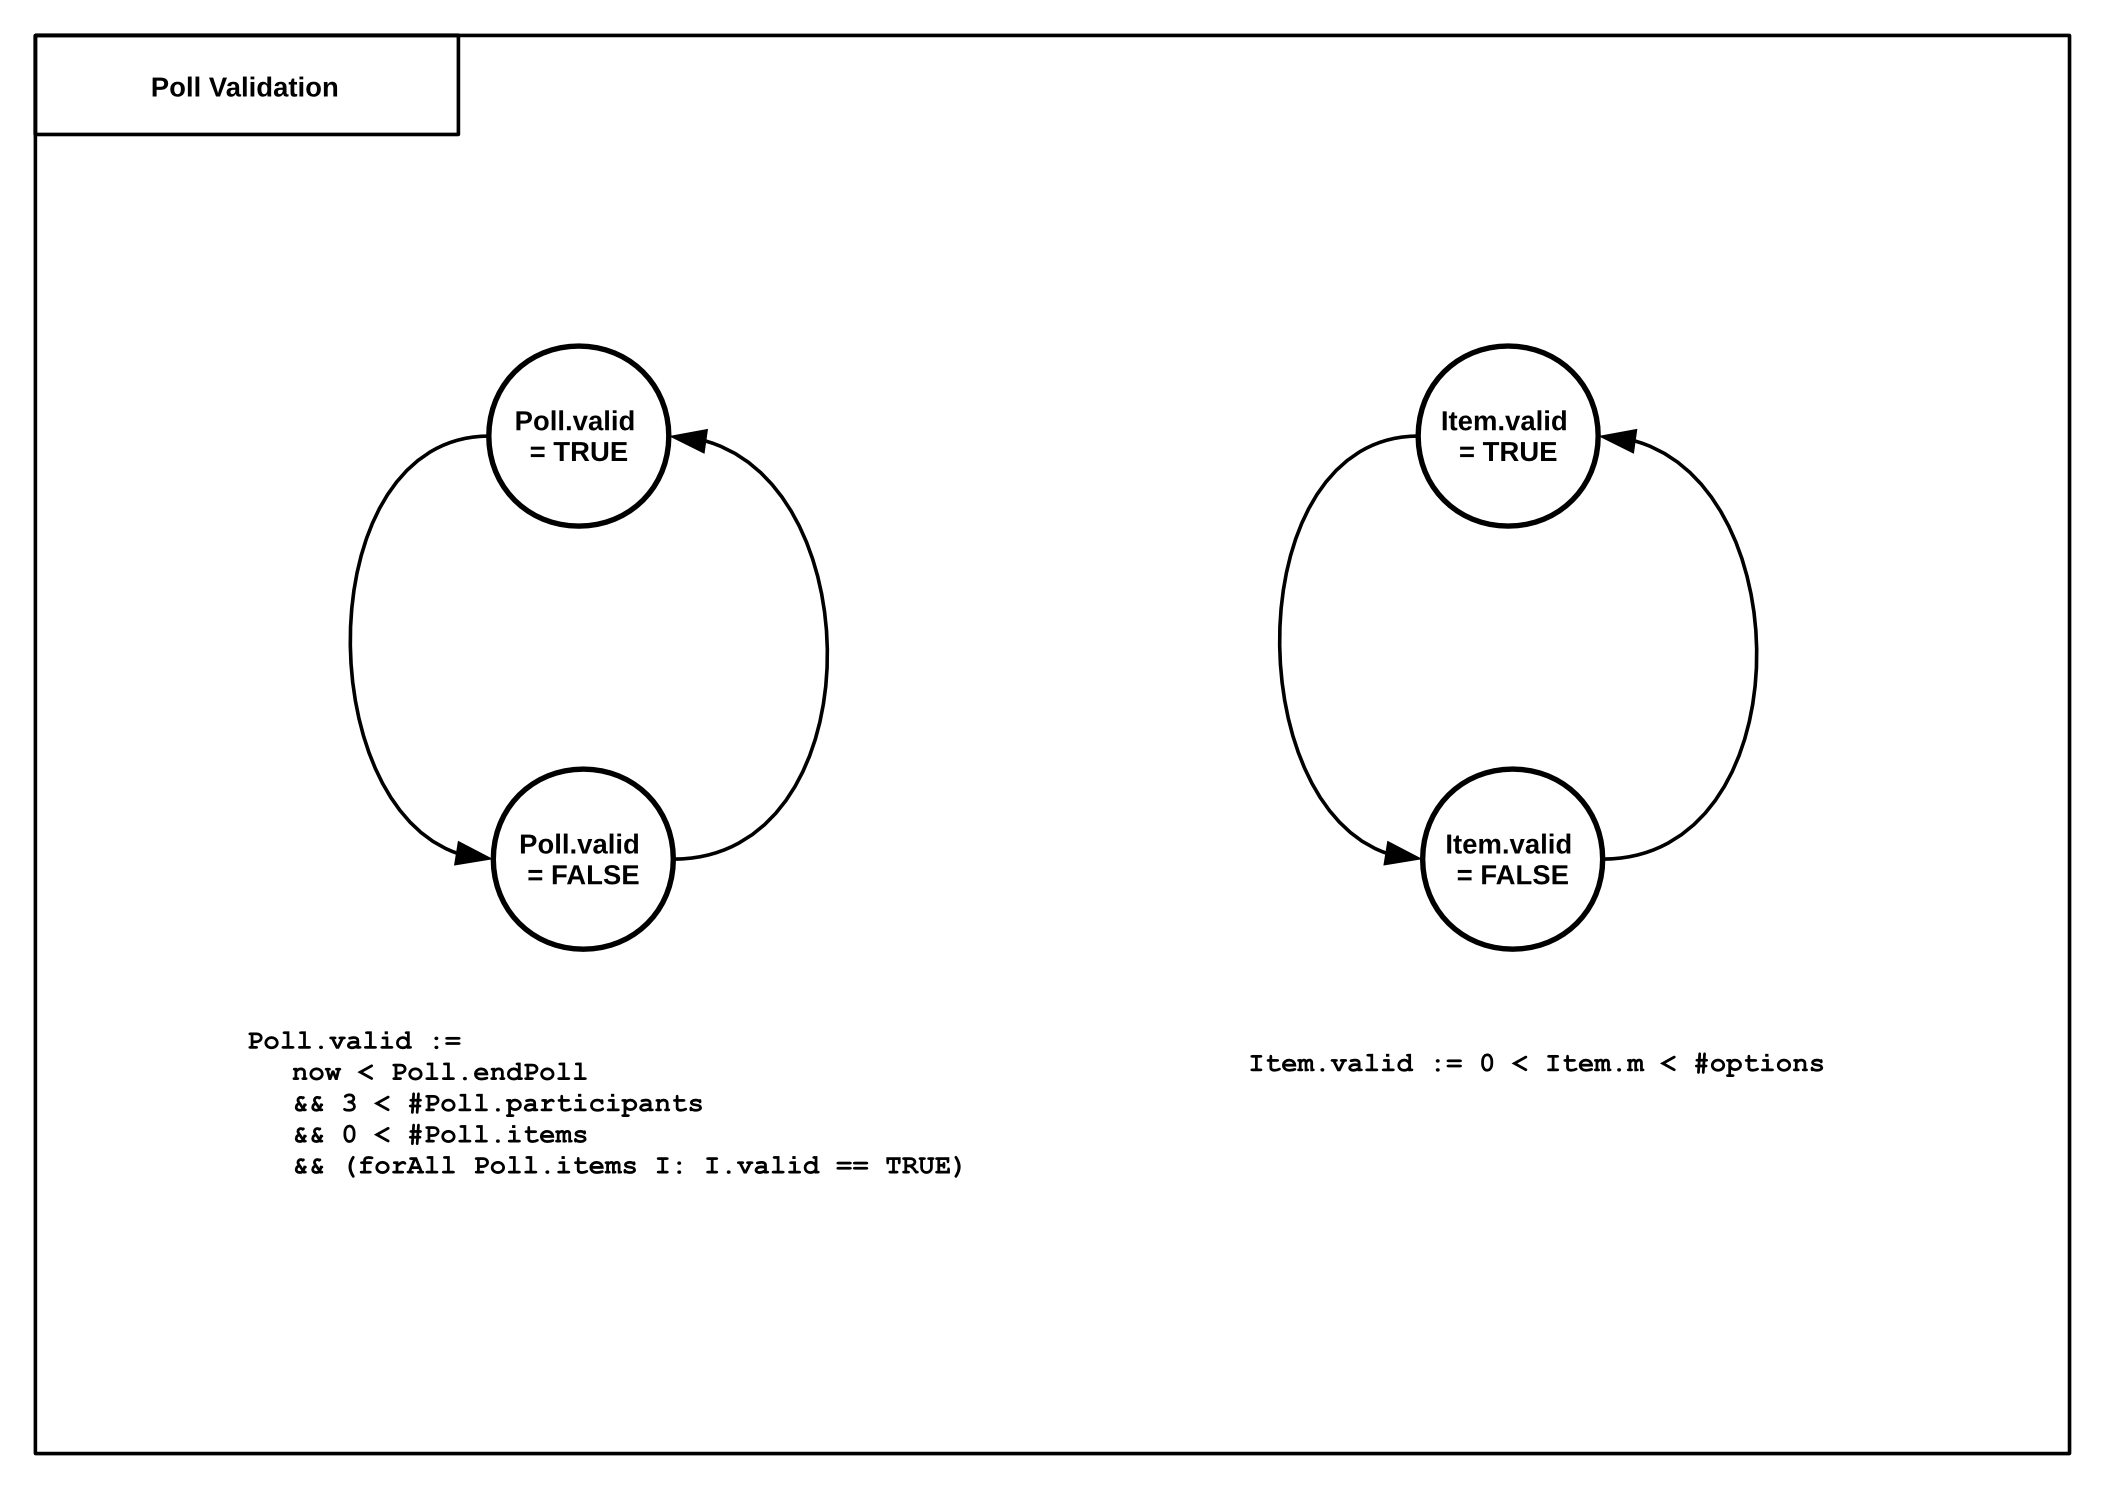
\includegraphics[width=0.7\textwidth]{png/poll-validation.png}
\caption{Poll Validation}
\label{figure:poll-validation}
\end{figure}

Another notable exception is the validation of polls, depicted in figure \ref{figure:poll-validation}.
Like the poll state, the poll valid flag is frequently updated when a poll is accessed.
Poll validation is one mean to ensure anonymity as only valid polls can be started.
For instance, a poll cannot be valid if less than three participants are defined.

However, such business operations are still closely related to CRUD.
So they are no additional business classes or packages besides the EJB facade, which is described in the following section.

\subsubsection{The VotesEJB Facade}
\label{subsubsec:the-votesejb-facade}
JavaEE Web Applications also encourage the use of the \textit{Facade}\footnote{\url{http://en.wikipedia.org/wiki/Facade_pattern}} pattern.
Facades in general are used to hide complexity by only making the relevant features available to the outside.
The facade of the VotesEJB module called \texttt{VotesLogic} is exemplified in figure \ref{figure:ejb-facade}.

\begin{figure}[h]
\centering
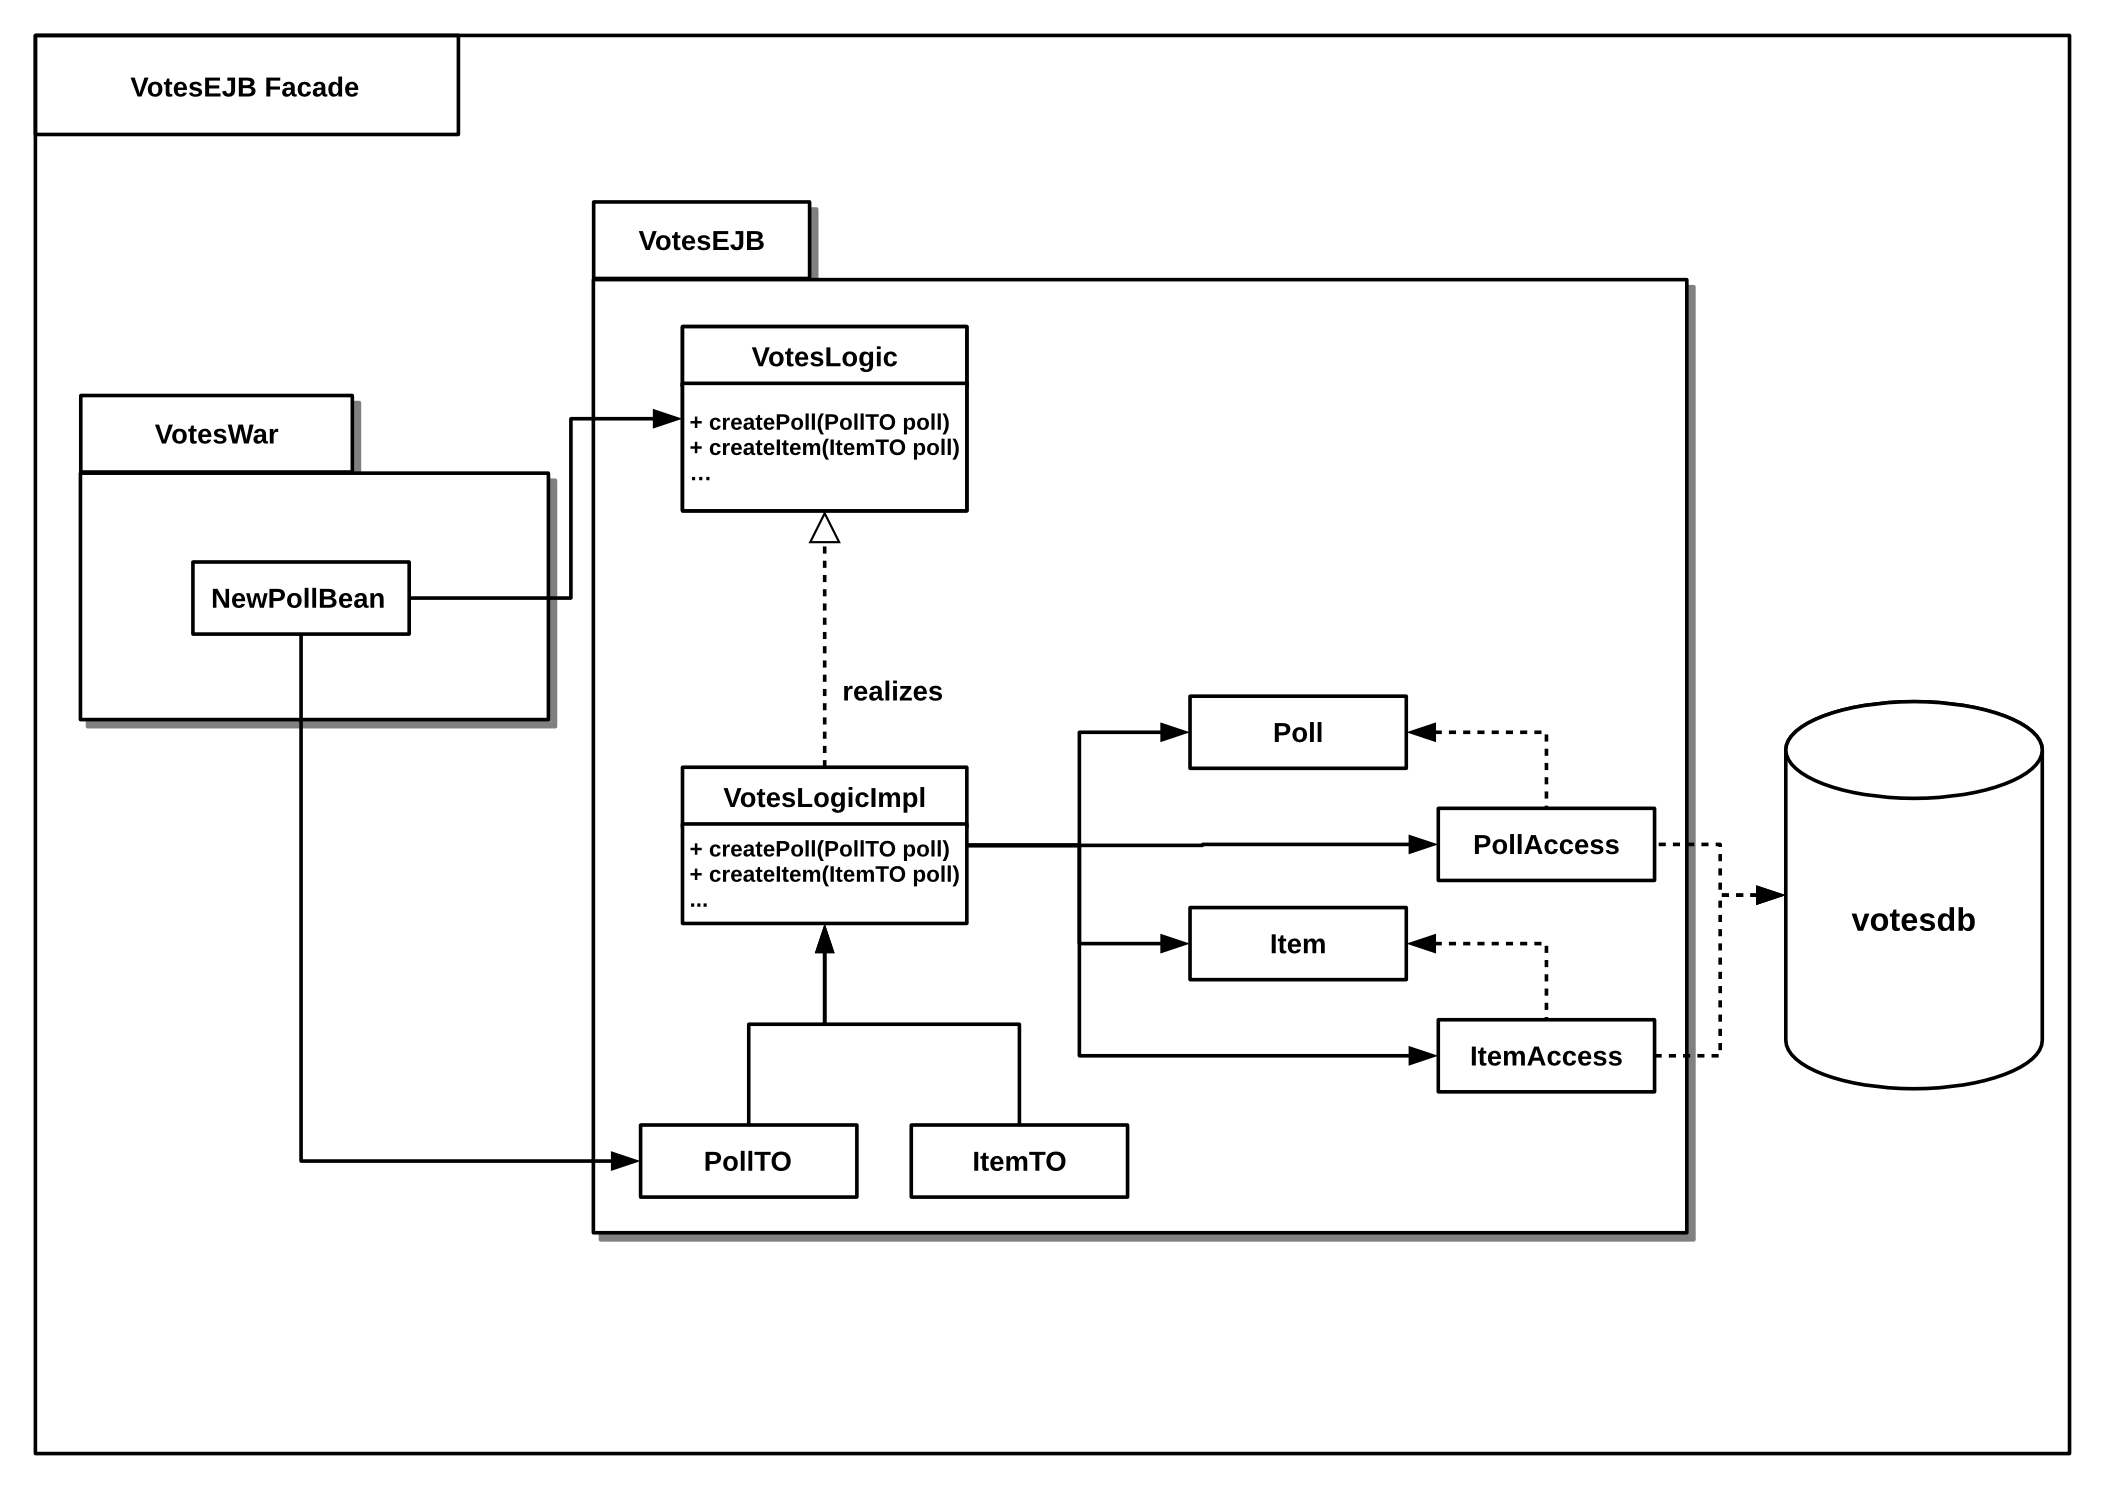
\includegraphics[width=0.7\textwidth]{png/ejb-facade.png}
\caption{VotesEJB Facade}
\label{figure:ejb-facade}
\end{figure}

The facade is used to handle communication between the VotesEJB and VotesWar modules.
Therefore, the class \texttt{VotesLogicImpl} is injected into beans of VotesWar.
The votes facade provides means to create, read, update and delete entities, and additional business logic methods such as poll validation and user authentication.
Figure \ref{figure:ejb-facade} also shows, that the facade internally uses the data mapper pattern described in section §\ref{subsubsec:votes-entity-persistence}.

Because the VotesEJB and VotesWar modules are instantiated separately, the communication is handled through \textit{Data Transfer Objects}\footnote{\url{http://martinfowler.com/eaaCatalog/dataTransferObject.html}} like \texttt{PollTO} instead of entity objects.
Such transfer objects exactly mirror the structure of entities, but provide a more lightweight form of serialization than entity objects as they do not contain additional mutators.



\subsection{VotesWar Architecture}
JavaEE Web Applications package presentation and user interface logic into WAR modules.
Votes makes use of the JavaServer Faces\footnote{\url{https://javaserverfaces.java.net/}} API (JSF) to create user interface components and their interactions.
In order to create a common look and feel, we use Twitter Bootstrap\footnote{\url{http://getbootstrap.com/}}.
Result charts a created by the Highcharts\footnote{\url{http://www.highcharts.com/}} API.
The outline of votes web pages is depicted in figure \ref{figure:web-directory-outline}.

\begin{figure}[h]
\centering
\begin{minipage}[t]{3cm}
\scriptsize
\begin{verbatim}
\resources
    \bootstrap
    \highcarts
    \jquery
    \votes
        \css
        \img
        \jsf
            ...
            \login.xhtml
            \navbar.xhtml
            ...
\edit-item.xhtml
\edit-poll.xhtml
\my-polls.xhtml
\new-poll.xhtml
\poll.xhtml
\register.xhtml
\result.xhtml
\end{verbatim}
\end{minipage}
\caption{VotesWar Web Pages Outline}
\label{figure:web-directory-outline}
\end{figure}

All top level XHTML files are accessible through navigation.
Additional resources are packaged into the \texttt{resources} directory.
Note that resources proprietary to votes also contain a \texttt{jsf} directory, containing reusable components, such as a login page or a navbar component.
The login page is only shown if needed to keep the web page as RESTful as possible.

JSF does not enforce any particular pattern as any bean is globally available inside the XHTML template notation.
However, we try to keep a 1:1-mapping between a backing bean and its corresponding web page if possible.
For instance, there is a file \texttt{NewPollBean} corresponding to the page \texttt{new-poll.xhtml}.
Exceptions are made for login handling. 
User information provided by a \texttt{UserBean} is used be various components.

Besides organizer registration, the votes web module handles two kinds of sessions.
That is: organizer sessions, which are used to administer polls.
And participation sessions, which handle the voting interactions of participants.
Both sessions are described in more detail by the following sections.



\subsubsection{Organizer Sessions}
An Organizer is able to create new polls or edit existing polls and their items.
The figure \ref{figure:web-organizer-navigation-graph} shows the navigation possibilities on the web-page. The page \texttt{my-polls} is the first page an organizer sees after he logged in. It is also the most central place because it is possible to navigate to \texttt{my-polls} from every page.
After the organizer created a new poll on the \texttt{new-poll} page he get directed to the \texttt{edit-poll} page where he can edit the attributes of a poll (Title, End-Date, etc.) and add new items and participants to the poll. By clicking on the title of an corresponding item the organizer navigates to \texttt{edit-item} page.



\begin{figure}[h]
\centering
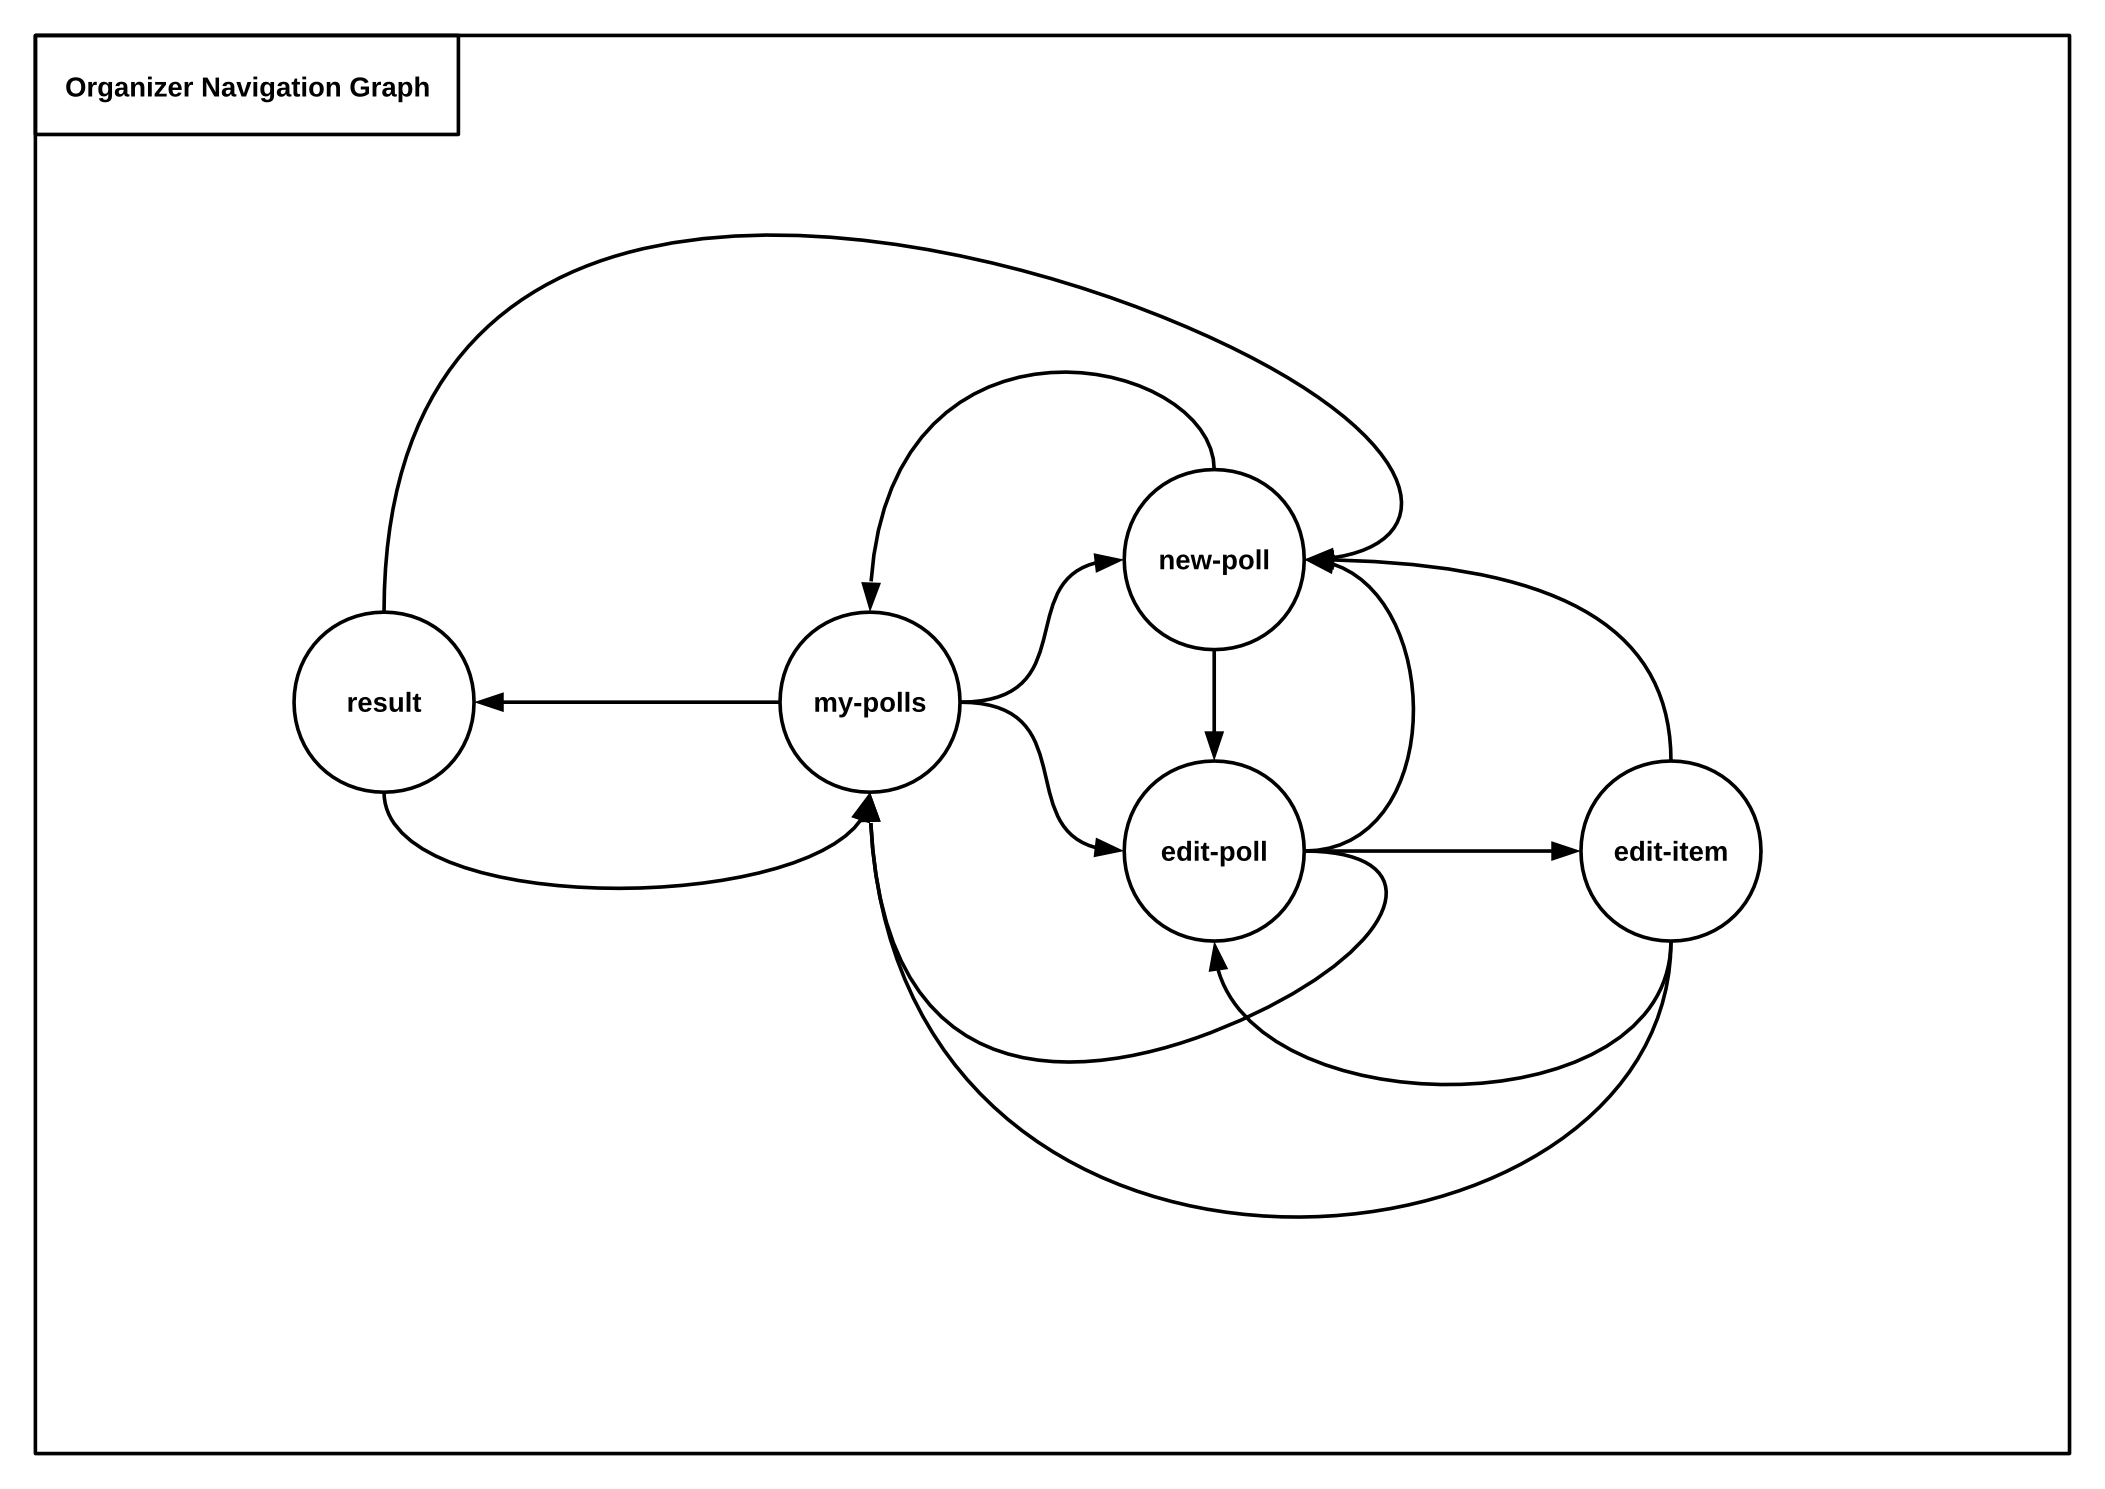
\includegraphics[width=0.7\textwidth]{png/web-organizer-navigation-graph.png}
\caption{VotesWar Organizer Navigation Graph}
\label{figure:web-organizer-navigation-graph}
\end{figure}

\subsubsection{Participant Sessions}
The figure \ref{figure:web-participation-state-machine} shows the pages which an participant of a poll sees when participating in  a poll. By inserting a valid token on the \texttt{Token-Verification} page a participant gets directed to the \texttt{Poll-Voting} page of the poll he got invited to. After he submitted the poll he gets directed to the \texttt{Token-Verification} page again.
\begin{figure}[h]
\centering
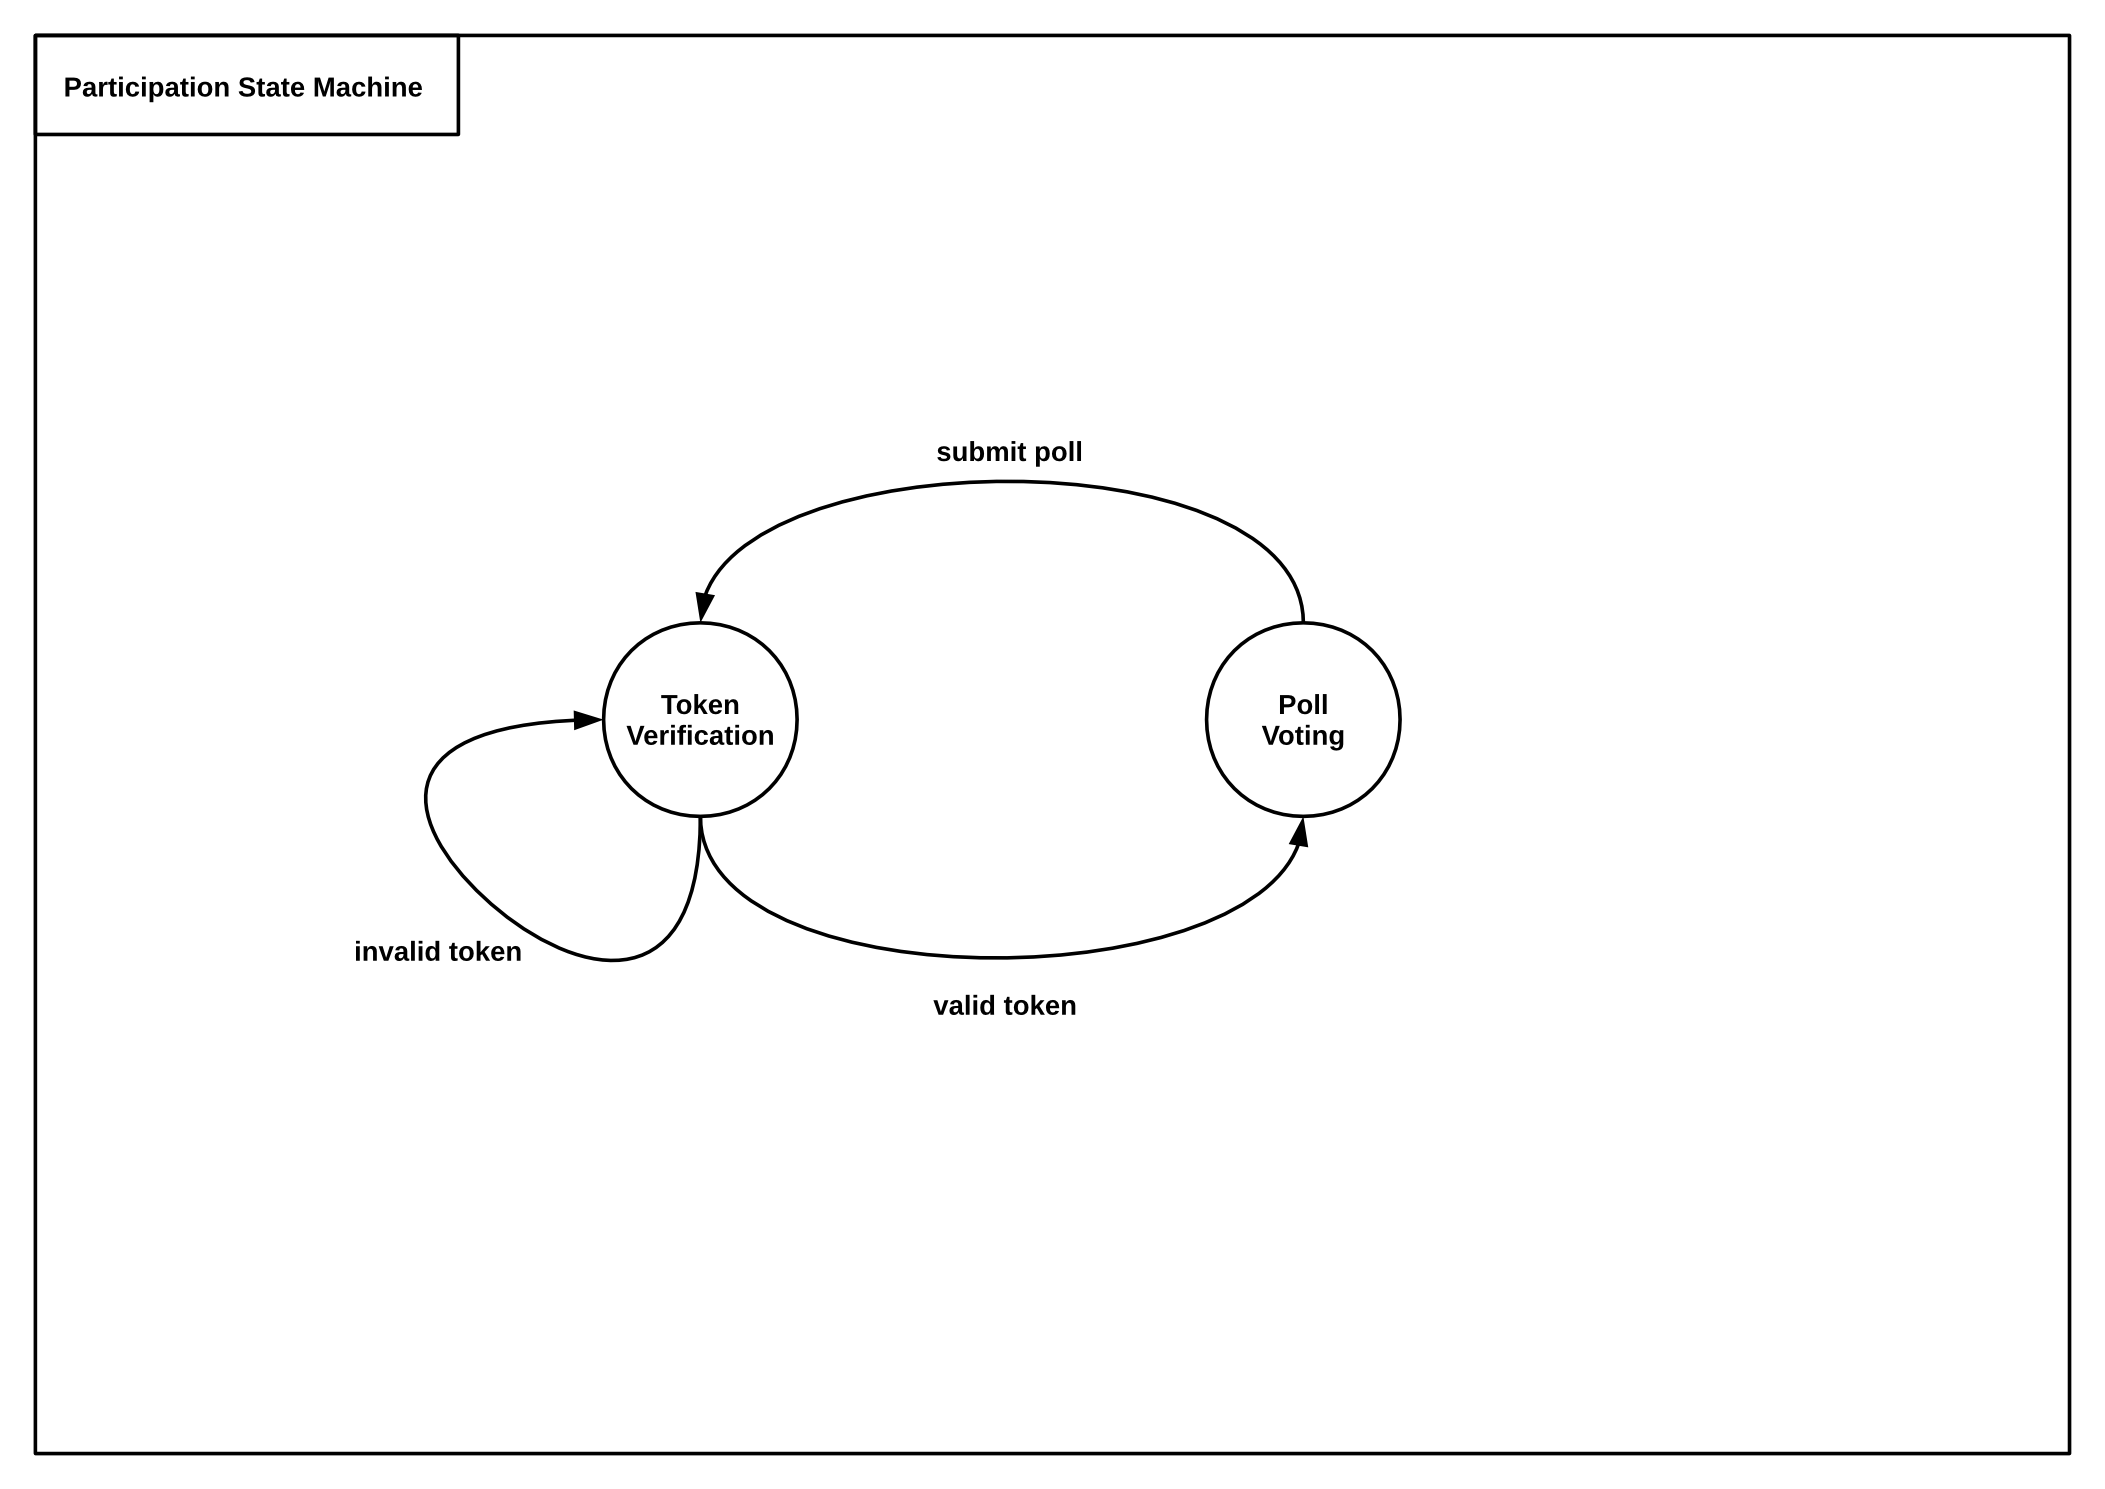
\includegraphics[width=0.7\textwidth]{png/web-participant-state-machine.png}
\caption{VotesWar Patricipation State Machine}
\label{figure:web-participation-state-machine}
\end{figure}




